% !TEX program = pdflatex
% Tufte-style manual for CurvilinearFilters

\documentclass[a4paper,justified]{tufte-book}

\usepackage{amsmath,amssymb}
\usepackage{graphicx}
\usepackage{booktabs}
\usepackage{hyperref}
\usepackage{listings}
\usepackage{xcolor}
\usepackage{tikz}
\usetikzlibrary{arrows.meta, positioning, shapes.geometric}

\definecolor{codegray}{rgb}{0.95,0.95,0.95}
\lstset{
	language=Matlab,
	backgroundcolor=\color{codegray},
	basicstyle=\ttfamily\small,
	frame=single,
	breaklines=true,
	columns=fullflexible
}

\title{Curvilinear Filters\\[0.5em]\large A MATLAB Reference Manual}
\author{ }
\date{ }

\begin{document}
\maketitle
\tableofcontents
\newpage

% =============================================================================
\section{Summary}
% =============================================================================

This manual documents the \texttt{CurvilinearFilters} package, a collection of
MATLAB modules for detecting and enhancing curvilinear structures in 2-D images
prior to segmentation. Five complementary filter families are covered:

\begin{description}
  \item[\textbf{Hessian}] Multiscale Hessian-based detectors (vesselness, ridge,
        blobness, plateness, neuriteness).
  \item[\textbf{MFAT}] Multiscale Fractional Anisotropy Tensor --- deterministic
        and probabilistic variants.
  \item[\textbf{Phase Congruency}] Log-Gabor filter bank edge/corner detector
        and phase symmetry measure.
  \item[\textbf{SOAGK}] Steerable Orientation-Aligned Gaussian Kernels, an
        anisotropic line detector.
  \item[\textbf{Vesselness (optimised)}] A standalone optimised implementation
        of the original Frangi vessel filter, retained as a legacy reference.
\end{description}

All modules share a common synthetic benchmark image and a unified figure
directory for reproducible documentation.

% =============================================================================
\section{Introduction}
% =============================================================================

Curvilinear structures---blood vessels, neurites, fibres, and reticular
networks---are ubiquitous in biological and industrial imaging. Their
reliable detection is a prerequisite for segmentation, tracing, and
quantification pipelines. No single filter is universally optimal: tubular
structures, ridge lines, and symmetric features each call for different
mathematical characterisations of local image geometry.

This package provides a curated set of filters that together span the major
design strategies: second-order differential analysis (Hessian family),
tensor-based fractional anisotropy (MFAT), Fourier-domain phase measurement
(Phase Congruency/Symmetry), and steerable filter banks (SOAGK). Each module
is implemented in clean, tested MATLAB with no toolbox dependencies beyond
the Image Processing Toolbox.

% =============================================================================
\section{Mathematical Background}
% =============================================================================

\subsection{The Hessian Matrix and Scale Space}

Given a greyscale image $I(x,y)$, the Hessian matrix at scale $\sigma$ is
\begin{equation}
  \mathbf{H}_\sigma = \sigma^2
  \begin{pmatrix}
    \partial_{xx} I_\sigma & \partial_{xy} I_\sigma \\
    \partial_{xy} I_\sigma & \partial_{yy} I_\sigma
  \end{pmatrix},
\end{equation}
where $I_\sigma = I * G_\sigma$ denotes Gaussian smoothing and the $\sigma^2$
factor provides Lindeberg's scale normalisation, enabling meaningful
cross-scale comparison of responses.

Let $\lambda_1$, $\lambda_2$ be the eigenvalues ordered by
$|\lambda_1| \le |\lambda_2|$. Their signs and ratio characterise local
structure:

\begin{figure}
  \centering
  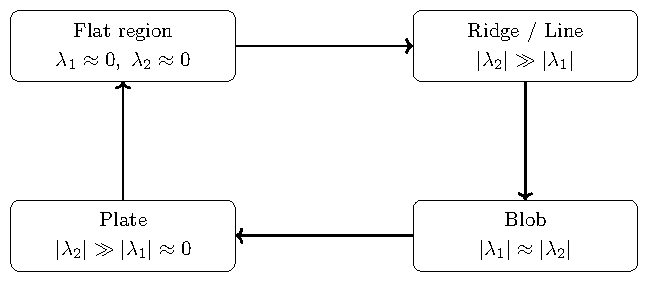
\includegraphics[width=\linewidth]{figures/hessian_geometry.pdf}
  \caption{Interpretation of Hessian eigenvalues in 2D: flat regions
  ($|\lambda_1| \approx |\lambda_2| \approx 0$), ridges
  ($|\lambda_2| \gg |\lambda_1|$, $\lambda_2 < 0$), and blobs
  ($|\lambda_1| \approx |\lambda_2|$, both negative).}
\end{figure}

The eigenvector corresponding to $\lambda_2$ points across a ridge; the
tangent direction is obtained by a $90^\circ$ rotation.

\subsection{Log-Gabor Filters and Phase Congruency}

Log-Gabor filters are band-pass filters constructed in the frequency domain:
\begin{equation}
  G(f) = \exp\!\left(\frac{-(\ln(f/f_0))^2}{2(\ln(\sigma_f))^2}\right),
\end{equation}
where $f_0$ is the centre frequency and $\sigma_f$ controls bandwidth.
A bank of log-Gabor filters at multiple scales and orientations decomposes
the image into oriented frequency sub-bands. Phase congruency measures the
degree to which these components are in phase at each location, providing an
illumination-invariant feature measure.

\subsection{Fractional Anisotropy}

In diffusion tensor imaging, fractional anisotropy (FA) quantifies the degree
to which diffusion is directionally asymmetric. MFAT adapts this concept to
image Hessian eigenvalues: a high FA-like score indicates a strongly
curvilinear (anisotropic) local geometry, independent of contrast magnitude.

% =============================================================================
\section{Hessian-Based Filters}
% =============================================================================

\subsection{Overview}

The Hessian module provides five filter types sharing a common low-level
numerical core (\texttt{applyHessian2D}, \texttt{eig2image}) and accessed
through a single entry-point function \texttt{hessian2DFilters}.

\begin{figure}
  \centering
  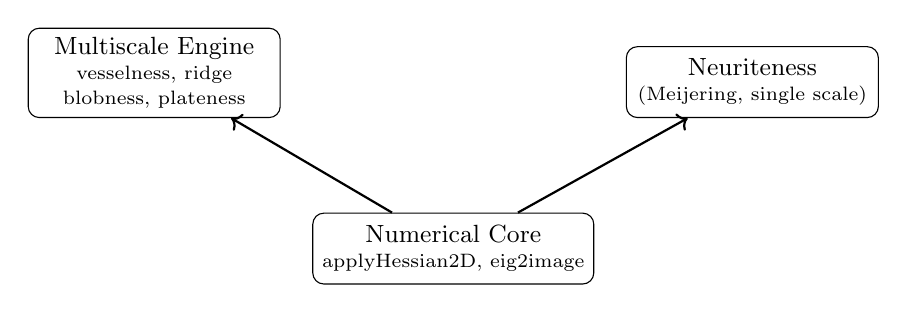
\begin{tikzpicture}[
    box/.style={draw, rounded corners, align=center, minimum width=3.2cm,
                minimum height=0.9cm, font=\small},
    arrow/.style={->, thick}
    ]
    \node[box] (core) {Numerical Core\\[-2pt]\scriptsize applyHessian2D, eig2image};
    \node[box, above left=1.2cm and 0.4cm of core]  (engine)
        {Multiscale Engine\\[-2pt]\scriptsize vesselness, ridge\\[-2pt]\scriptsize blobness, plateness};
    \node[box, above right=1.2cm and 0.4cm of core] (neurite)
        {Neuriteness\\[-2pt]\scriptsize (Meijering, single scale)};
    \draw[arrow] (core) -- (engine);
    \draw[arrow] (core) -- (neurite);
  \end{tikzpicture}
  \caption{Software architecture of the Hessian module. The numerical core is
  shared between the multiscale engine and the single-scale neuriteness filter.}
\end{figure}

\subsection{API}

\begin{lstlisting}
[R, scale, direction] = hessian2DFilters(I, ...)
%  'FilterType'  'vesselness' | 'ridge' | 'blob' | 'plate'
%  'Sigmas'      vector of scales (default: auto-computed)
%  'WhiteOnDark' true | false (default: true)
%  'Precision'   'single' | 'double' (default: 'single')
%  'Parameters'  struct with filter-specific overrides

[N, direction] = neuriteness2D(I, sigma)
\end{lstlisting}

\subsection{Vesselness (Frangi, 1998)}

The vesselness response at scale $\sigma$ combines Hessian eigenvalues
into a score that rewards elongated, tubular geometry:
\begin{align}
  \mathcal{R}_B &= \frac{\lambda_1}{\lambda_2}, \\
  S^2 &= \lambda_1^2 + \lambda_2^2, \\
  V_\sigma &= \exp\!\left(\frac{-\mathcal{R}_B^2}{2\beta^2}\right)
              \left(1 - \exp\!\left(\frac{-S^2}{2c^2}\right)\right),
\end{align}
with defaults $\beta = 0.5$, $c = 15$. The final response is
$V(x) = \max_{\sigma} V_\sigma(x)$.

\subsection{Ridge Filter (Sato, 1998)}

The ridge response rewards line-like structures by penalising blob-like
responses via the ratio $\lambda_1/\lambda_2$.

\subsection{Blobness (Lindeberg, 1998)}

Blobness uses the normalised determinant of the Hessian:
$B = \lambda_1 \lambda_2$.

\subsection{Plateness}

The 2-D plateness measure detects thick elongated regions with low curvature
anisotropy, analogous to the plate measure used in 3-D analysis.

\subsection{Neuriteness (Meijering et al., 2004)}

Modified eigenvalues are formed as
$\tilde{\lambda}_1 = \lambda_1 + \alpha\lambda_2$,
$\tilde{\lambda}_2 = \lambda_2 + \alpha\lambda_1$,
with $\alpha = -1/3$, then reordered by magnitude. The response
\begin{equation}
  N(x) =
  \begin{cases}
    \tilde{\lambda}_1(x) / \min_x(\tilde{\lambda}_1), & \tilde{\lambda}_1(x) < 0, \\
    0, & \text{otherwise},
  \end{cases}
\end{equation}
yields a normalised, contrast-invariant, single-scale measure in $[0,1]$.

\subsection{Results}

\begin{figure*}[ht]
  \centering
  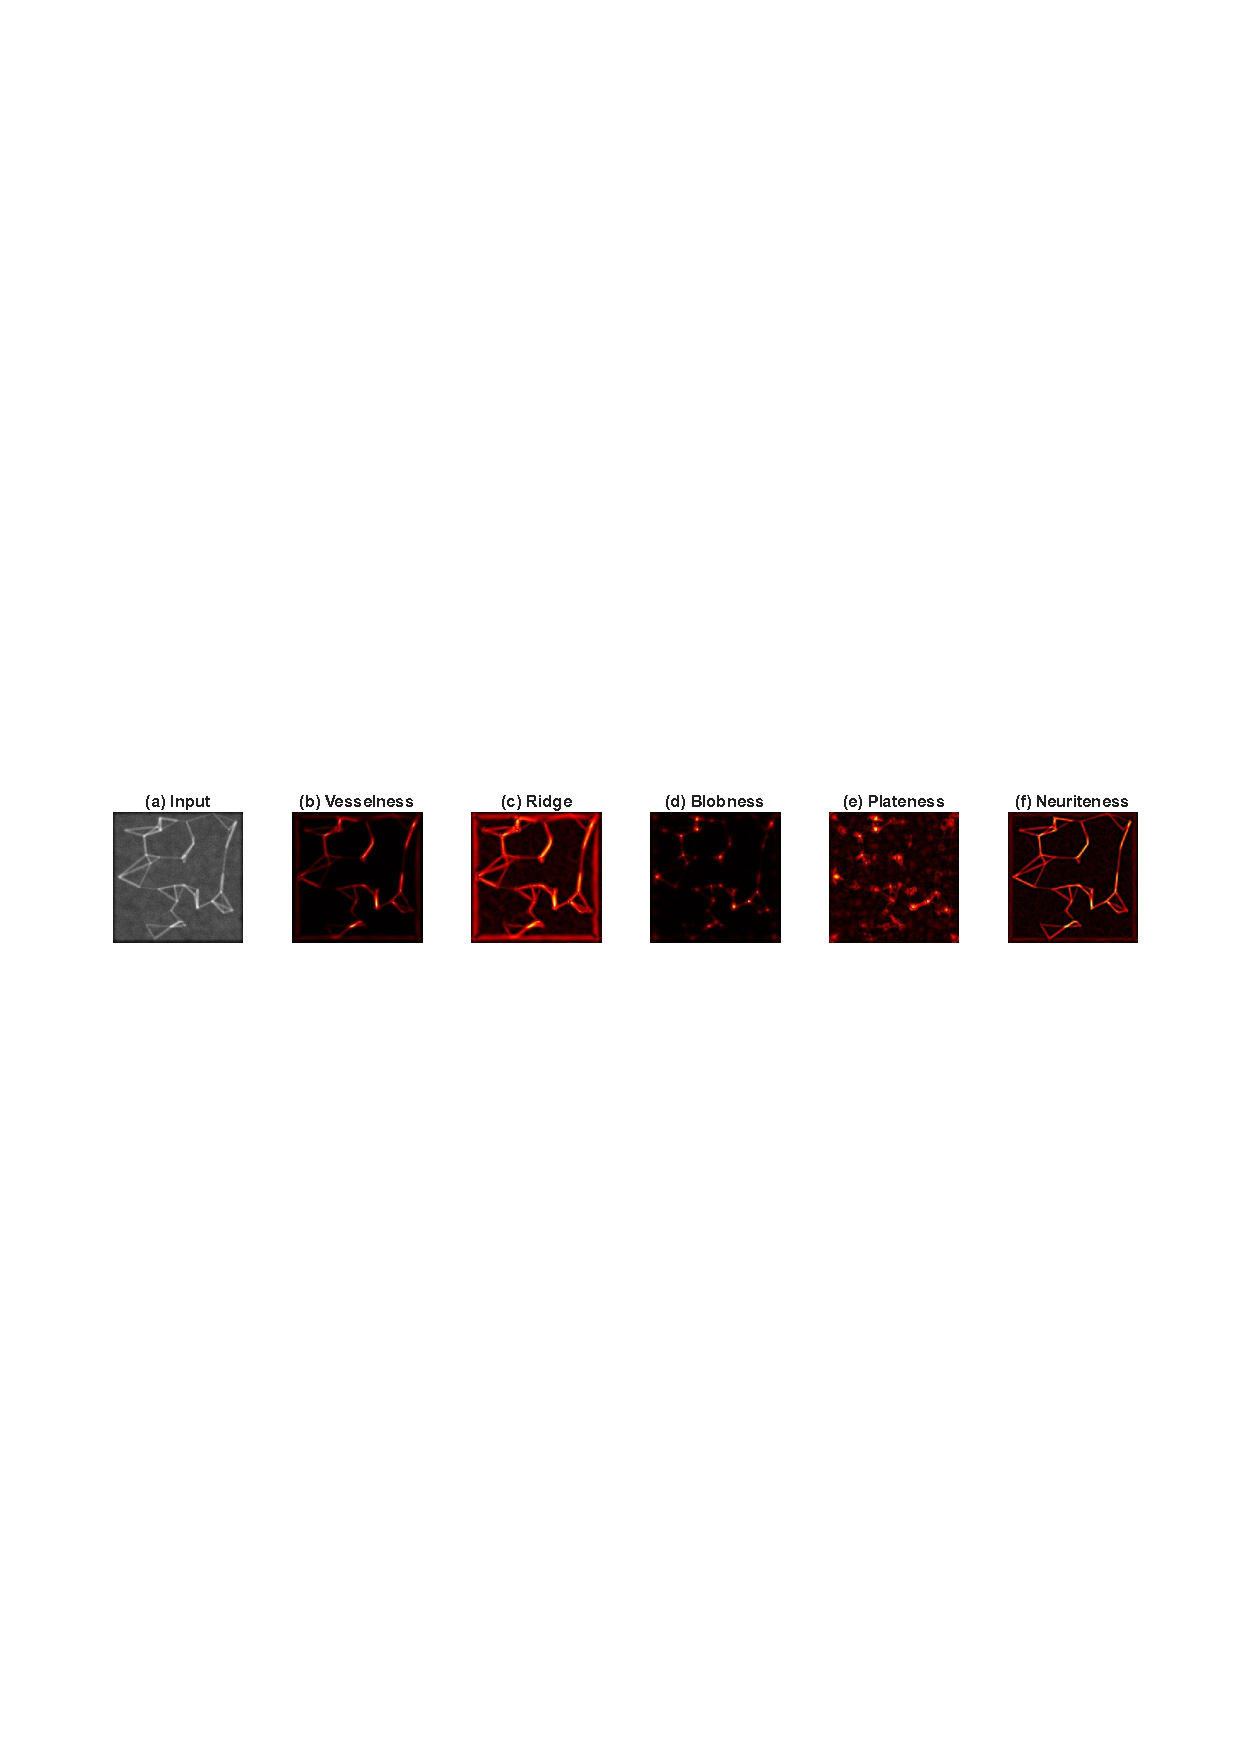
\includegraphics[width=\linewidth]{figures/hessian_composite.pdf}
  \caption{Hessian module responses on the reticulate benchmark image.
  (a)~Input. (b)~Vesselness. (c)~Ridge. (d)~Blobness. (e)~Plateness.
  (f)~Neuriteness. Observe that vesselness and ridge emphasise fine
  tubular segments, while neuriteness suppresses blob-like junction pixels.}
\end{figure*}

\newpage

% =============================================================================
\section{MFAT --- Multiscale Fractional Anisotropy Tensor}
% =============================================================================

\subsection{Overview}

MFAT adapts the fractional anisotropy (FA) concept from diffusion MRI to
2-D image analysis \cite{Alhasson2018}. Two complementary outputs are provided:

\begin{description}
  \item[\textbf{MFAT-$\lambda$}] Deterministic backbone. Produces a near-binary
        evidence map via strict post-processing rules.
  \item[\textbf{MFAT-Prob}] Probabilistic extension. Accumulates
        Beta-distributed likelihoods across scales and returns a posterior
        probability in $[0,1]$.
\end{description}

Optional modifiers (\texttt{mfatEntropyWeight}, \texttt{mfatFractional})
adjust the response for uncertain or weak-signal regions.

\subsection{API}

\begin{lstlisting}
out = mfatLambda(I, sigmas, ...)
%  'tau'         lower eigenvalue clipping factor (default: 0.03)
%  'tau2'        upper eigenvalue clipping factor (default: 0.30)
%  'D'           aggregation strength (default: 0.27)
%  'whiteOnDark' true | false (default: true)
%  'precision'   'single' | 'double' (default: 'single')

out = mfatProb(I, sigmas, ...)   % same parameters
\end{lstlisting}

\subsection{Algorithm: MFAT-$\lambda$}

For each scale $\sigma$:
\begin{enumerate}
  \item Compute scale-normalised Hessian eigenvalues $\lambda_1, \lambda_2$.
  \item Apply three-factor regularisation (clipping at $\tau$ and $\tau_2$).
  \item Compute the FA-like tensor measure:
        \begin{equation}
          \mathrm{FA} = \frac{|\lambda_2 - \lambda_1|}{
                              \sqrt{\lambda_1^2 + \lambda_2^2 + \varepsilon}}.
        \end{equation}
  \item Apply strict post-processing: response $\leftarrow 0$ if either
        eigenvalue $\ge 0$; aggregate via $D\tanh(\cdot - D) + \max$ fusion.
\end{enumerate}

\subsection{Algorithm: MFAT-Prob}

For each scale $\sigma$, model the MFAT-$\lambda$ response via Beta
likelihoods:
\begin{align}
  p_{\mathrm{vessel}}(r) &= \mathrm{Beta}(r;\, 2, 1), \\
  p_{\mathrm{bg}}(r)     &= \mathrm{Beta}(r;\, 1, 2).
\end{align}
Accumulate log-likelihood ratios across scales, then convert via a logistic
transform: $P(x) = (1 + \exp(-\mathrm{LLR}(x)))^{-1}$.

\subsection{Results}

\begin{figure*}[ht]
  \centering
  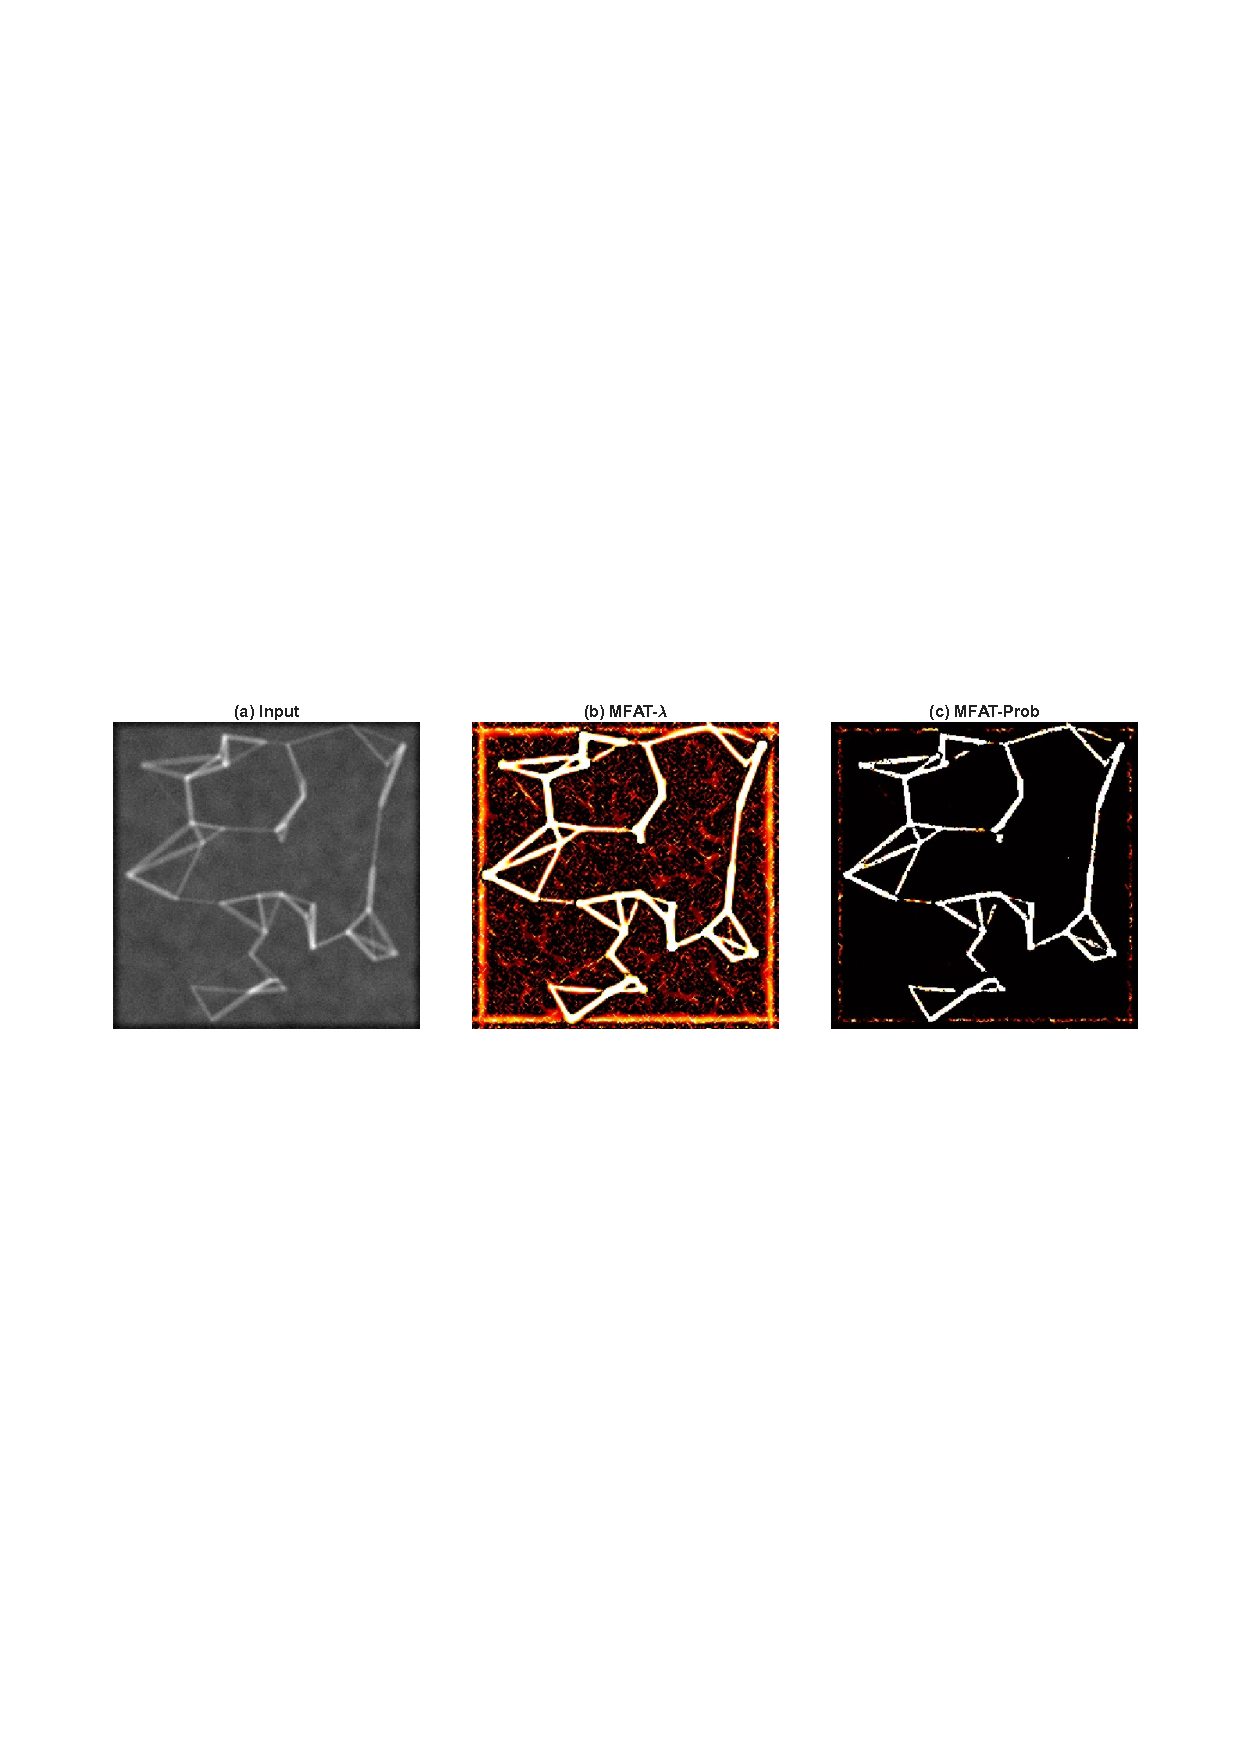
\includegraphics[width=0.9\linewidth]{figures/mfat_result.pdf}
  \caption{MFAT responses on the reticulate benchmark image.
  (a)~Input. (b)~MFAT-$\lambda$ (near-binary deterministic map).
  (c)~MFAT-Prob (posterior probability).}
\end{figure*}

\newpage

% =============================================================================
\section{Phase Congruency and Phase Symmetry}
% =============================================================================

\subsection{Overview}

Phase congruency \cite{Kovesi1999} measures feature strength as the degree to
which log-Gabor sub-bands are in phase, making it invariant to image contrast.
Phase symmetry extends this to detect symmetric (line-like and blob-like)
patterns. Both are implemented as optimised MATLAB functions with persistent
filter caches for efficiency.

\subsection{API}

\begin{lstlisting}
[M, m, or, featType, PC, EO, T, pcSum, noiseMask] = ...
    phaseCong3Optimised(I, ...)
%  'nscale'         number of scales (default: 4)
%  'norient'        number of orientations (default: 6)
%  'minWaveLength'  smallest scale wavelength (default: 5)
%  'mult'           scaling between successive filters (default: 2.1)
%  'sigmaOnf'       s.d.-to-centre-frequency ratio (default: 0.55)
%  'k'              noise threshold parameter (default: 2.0)
%  'precision'      'single' | 'double' | 'like' (default: 'double')

[phaseSym, orientation, totalEnergy, T] = phaseSymOptimised(I, ...)
%  'polarity'  1 (bright) | -1 (dark) | 0 (both, default)
\end{lstlisting}

\subsection{Phase Congruency}

At each point $x$, PC is the weighted ratio of aligned energy to total
filter response energy across all scales and orientations. Key outputs:

\begin{description}
  \item[$M$] Maximum moment of the PC covariance matrix (edge strength).
  \item[$m$] Minimum moment (corner/junction strength).
  \item[$\mathrm{or}$] Local orientation, in degrees $[0, 180)$.
\end{description}

\subsection{Phase Symmetry}

Phase symmetry sums the weighted phase alignment across orientations for
each scale, with polarity control allowing detection of bright, dark, or
both types of symmetric features.

\subsection{Results}

\begin{figure*}[ht]
  \centering
  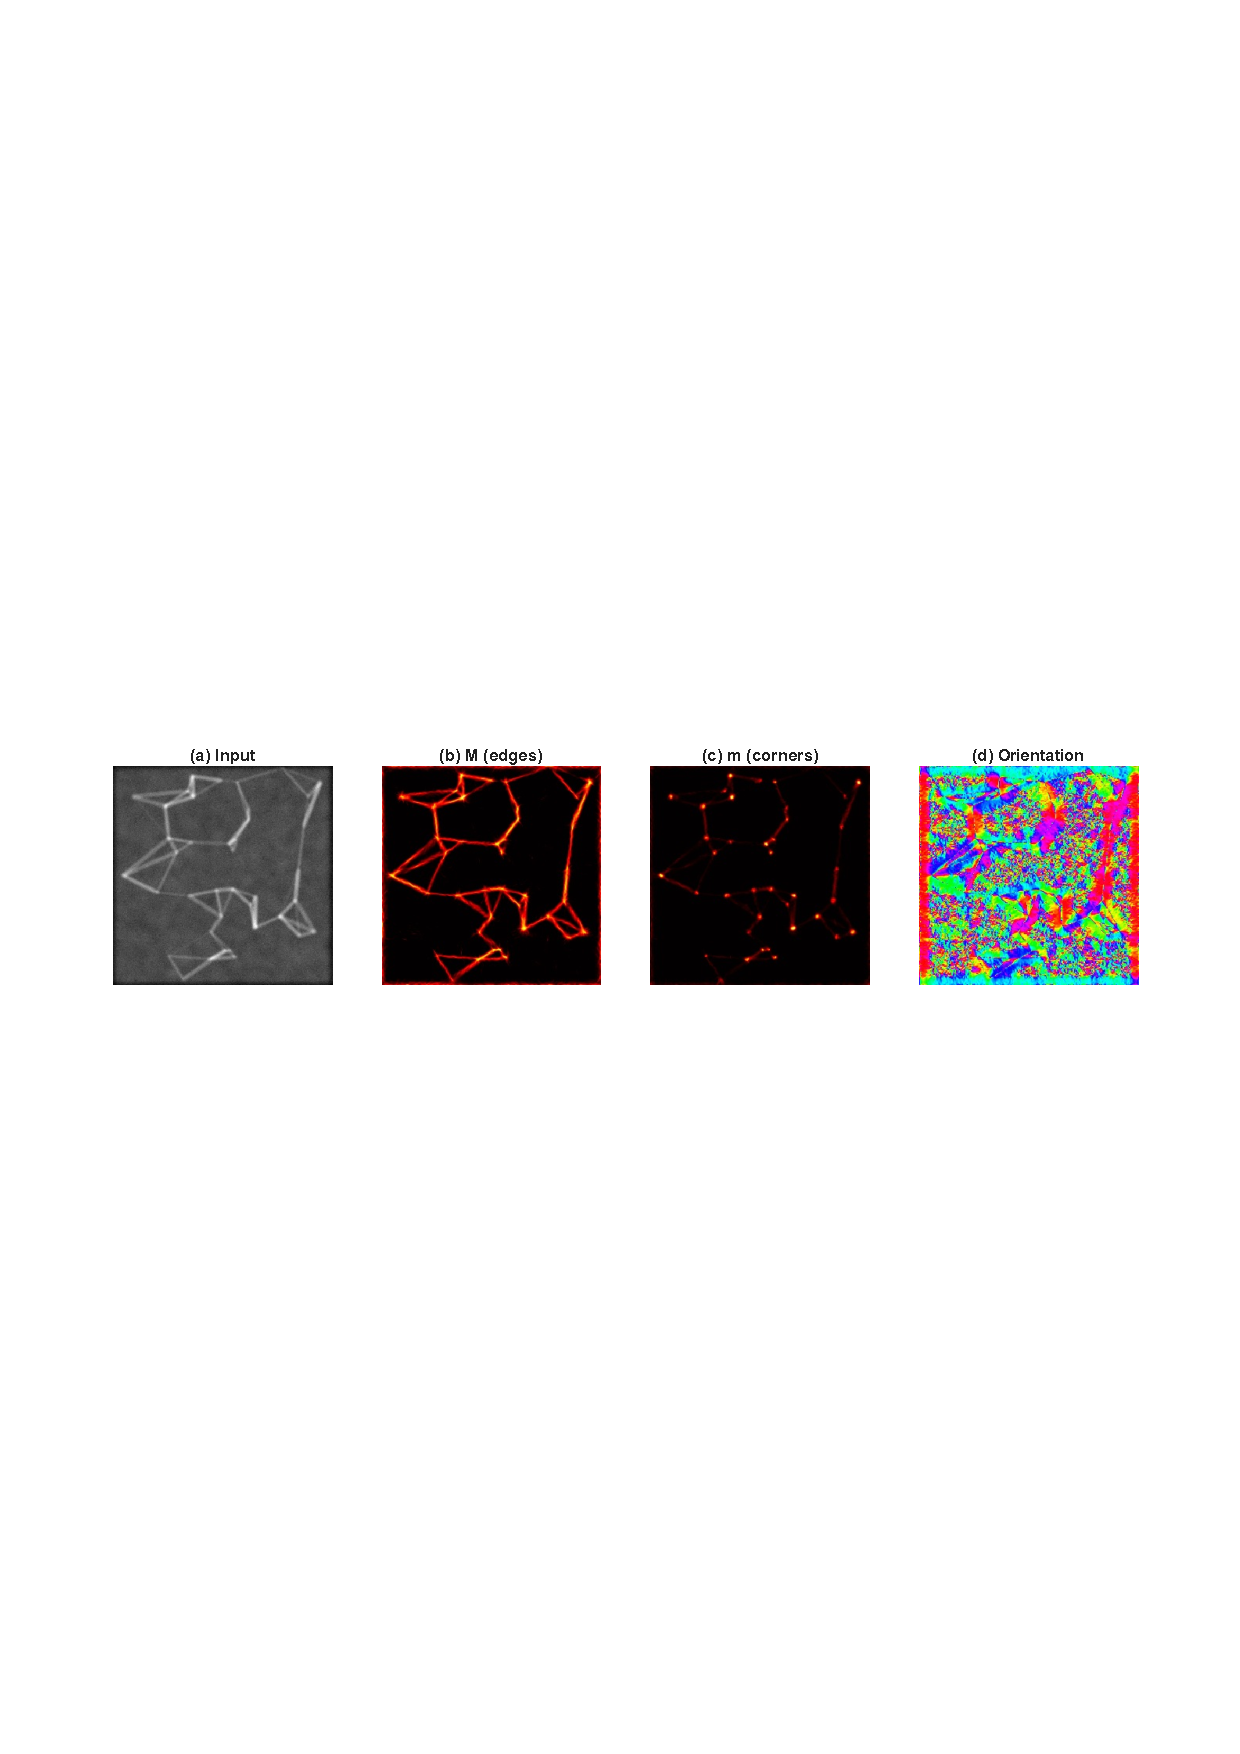
\includegraphics[width=\linewidth]{figures/phaseCongruency_result.pdf}
  \caption{Phase congruency on the reticulate benchmark image.
  (a)~Input. (b)~$M$ (edge map). (c)~$m$ (corner/junction map).
  (d)~Orientation (HSV colourmap).}
\end{figure*}

\begin{figure}
  \centering
  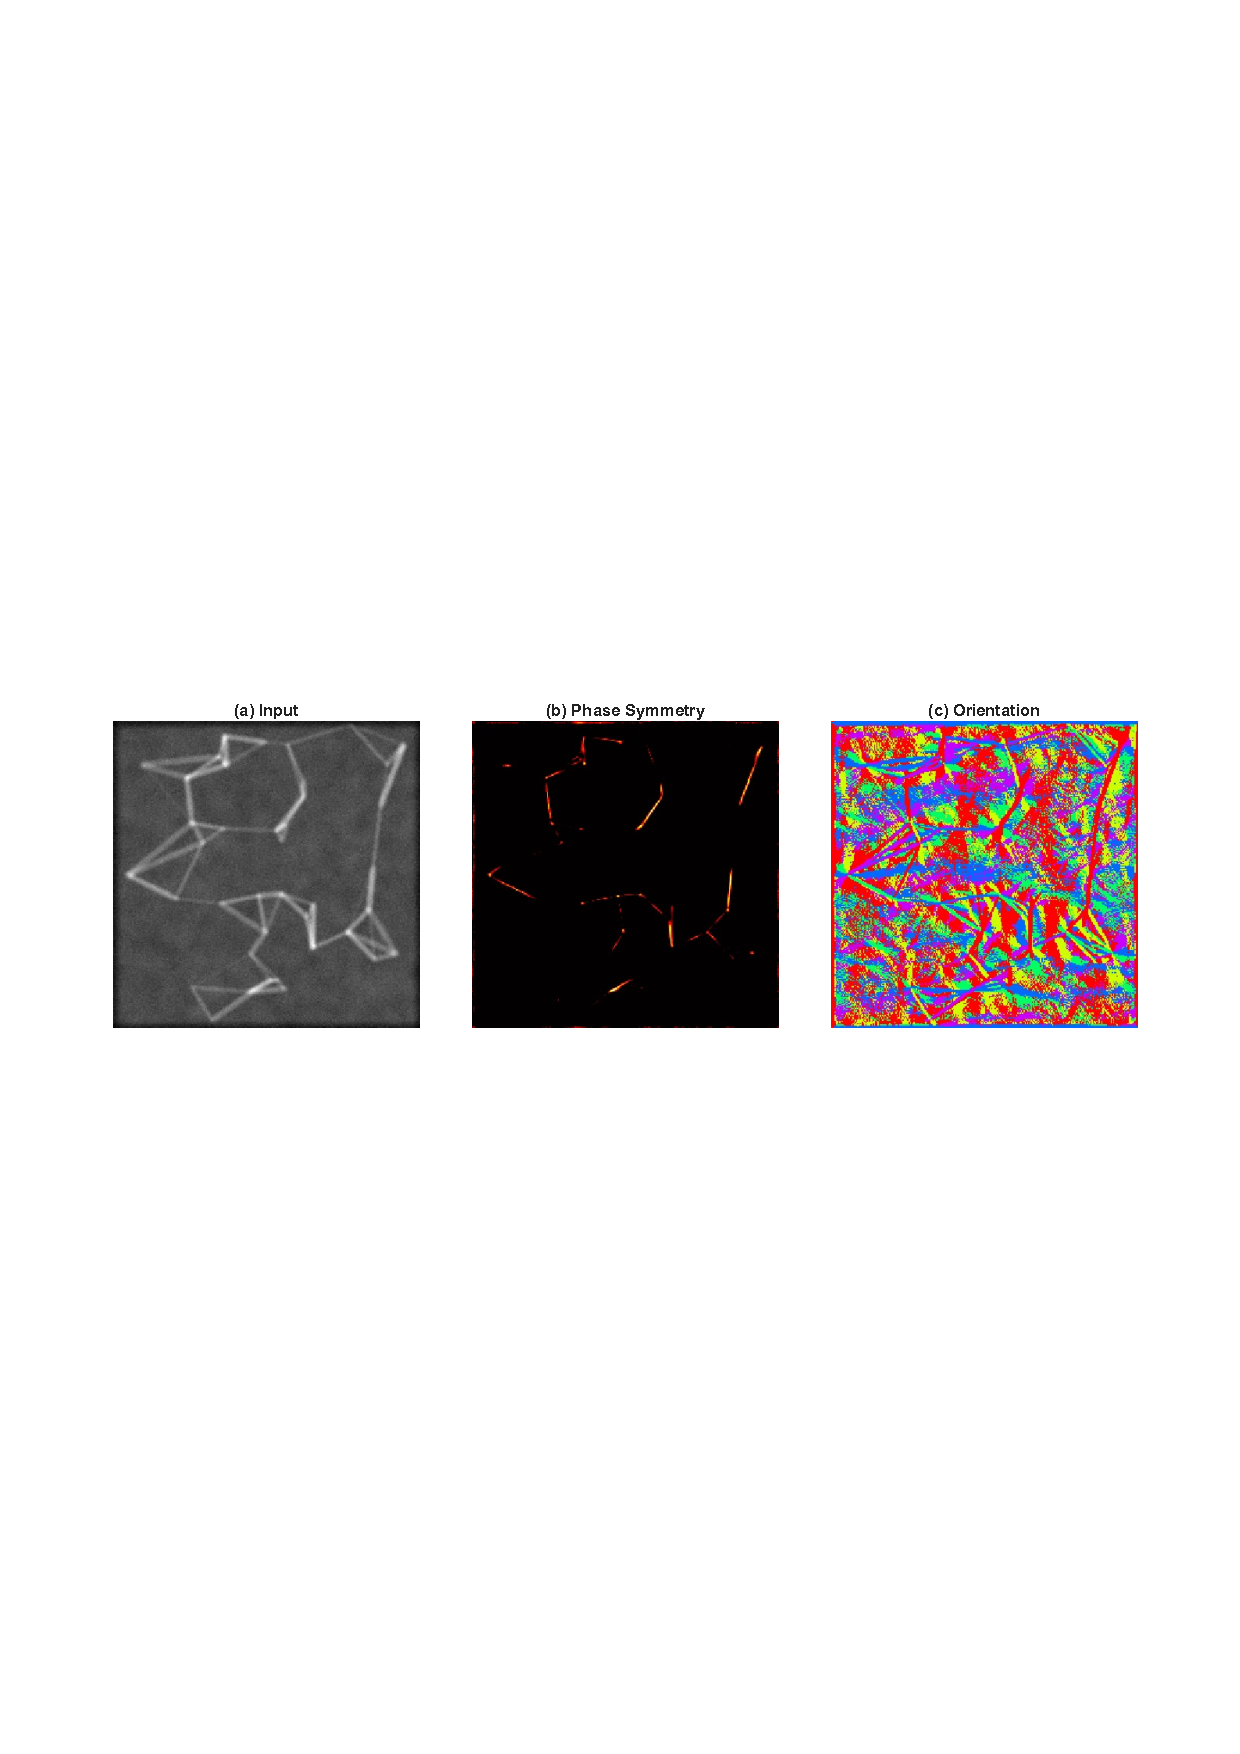
\includegraphics[width=\linewidth]{figures/phaseSymmetry_result.pdf}
  \caption{Phase symmetry on the reticulate benchmark image.
  (a)~Input. (b)~Symmetry response. (c)~Orientation.}
\end{figure}

\newpage

% =============================================================================
\section{SOAGK --- Steerable Orientation-Aligned Gaussian Kernels}
% =============================================================================

\subsection{Overview}

SOAGK implements a steerable anisotropic Gaussian line detector. A basis of
second-order anisotropic Gaussian derivative kernels is computed once per
scale/anisotropy pair and then steered analytically across orientations,
avoiding redundant convolutions.

\subsection{API}

\begin{lstlisting}
[lineMap, dirMap] = AGlineDetectorSteerableConv2( ...
    im, sigmas, thetas, rhos, precision)
%  im        grayscale image in [0, 1]
%  sigmas    vector of scales
%  thetas    orientations in [0, pi)
%  rhos      anisotropy factors >= 1
%  precision 'single' | 'double' (default: 'single')
%
%  lineMap   line strength in [0, 1]
%  dirMap    dominant orientation (radians)
\end{lstlisting}

An \texttt{imfilter}-based variant (\texttt{AGlineDetectorSteerable}) is also
provided and produces numerically equivalent results.

\subsection{Algorithm}

\begin{enumerate}
  \item For each $(\sigma, \rho)$ pair, construct the steerable basis
        $\{G_{xx}, G_{yy}, G_{xy}\}$ of anisotropic second-order Gaussian
        derivatives in the stretched coordinate frame
        $(x' = \rho x,\; y' = y/\rho)$.
  \item Convolve the image with each basis kernel once.
  \item For each orientation $\theta$, steer the response:
        \begin{equation}
          R_\theta = \cos^2\!\theta\; (G_{xx} * I)
                   + \sin^2\!\theta\; (G_{yy} * I)
                   + 2\cos\theta\sin\theta\; (G_{xy} * I).
        \end{equation}
  \item Retain $\max_{\sigma,\rho,\theta} R_\theta$ at each pixel and
        normalise to $[0,1]$.
\end{enumerate}

\subsection{Results}

\begin{figure*}[ht]
  \centering
  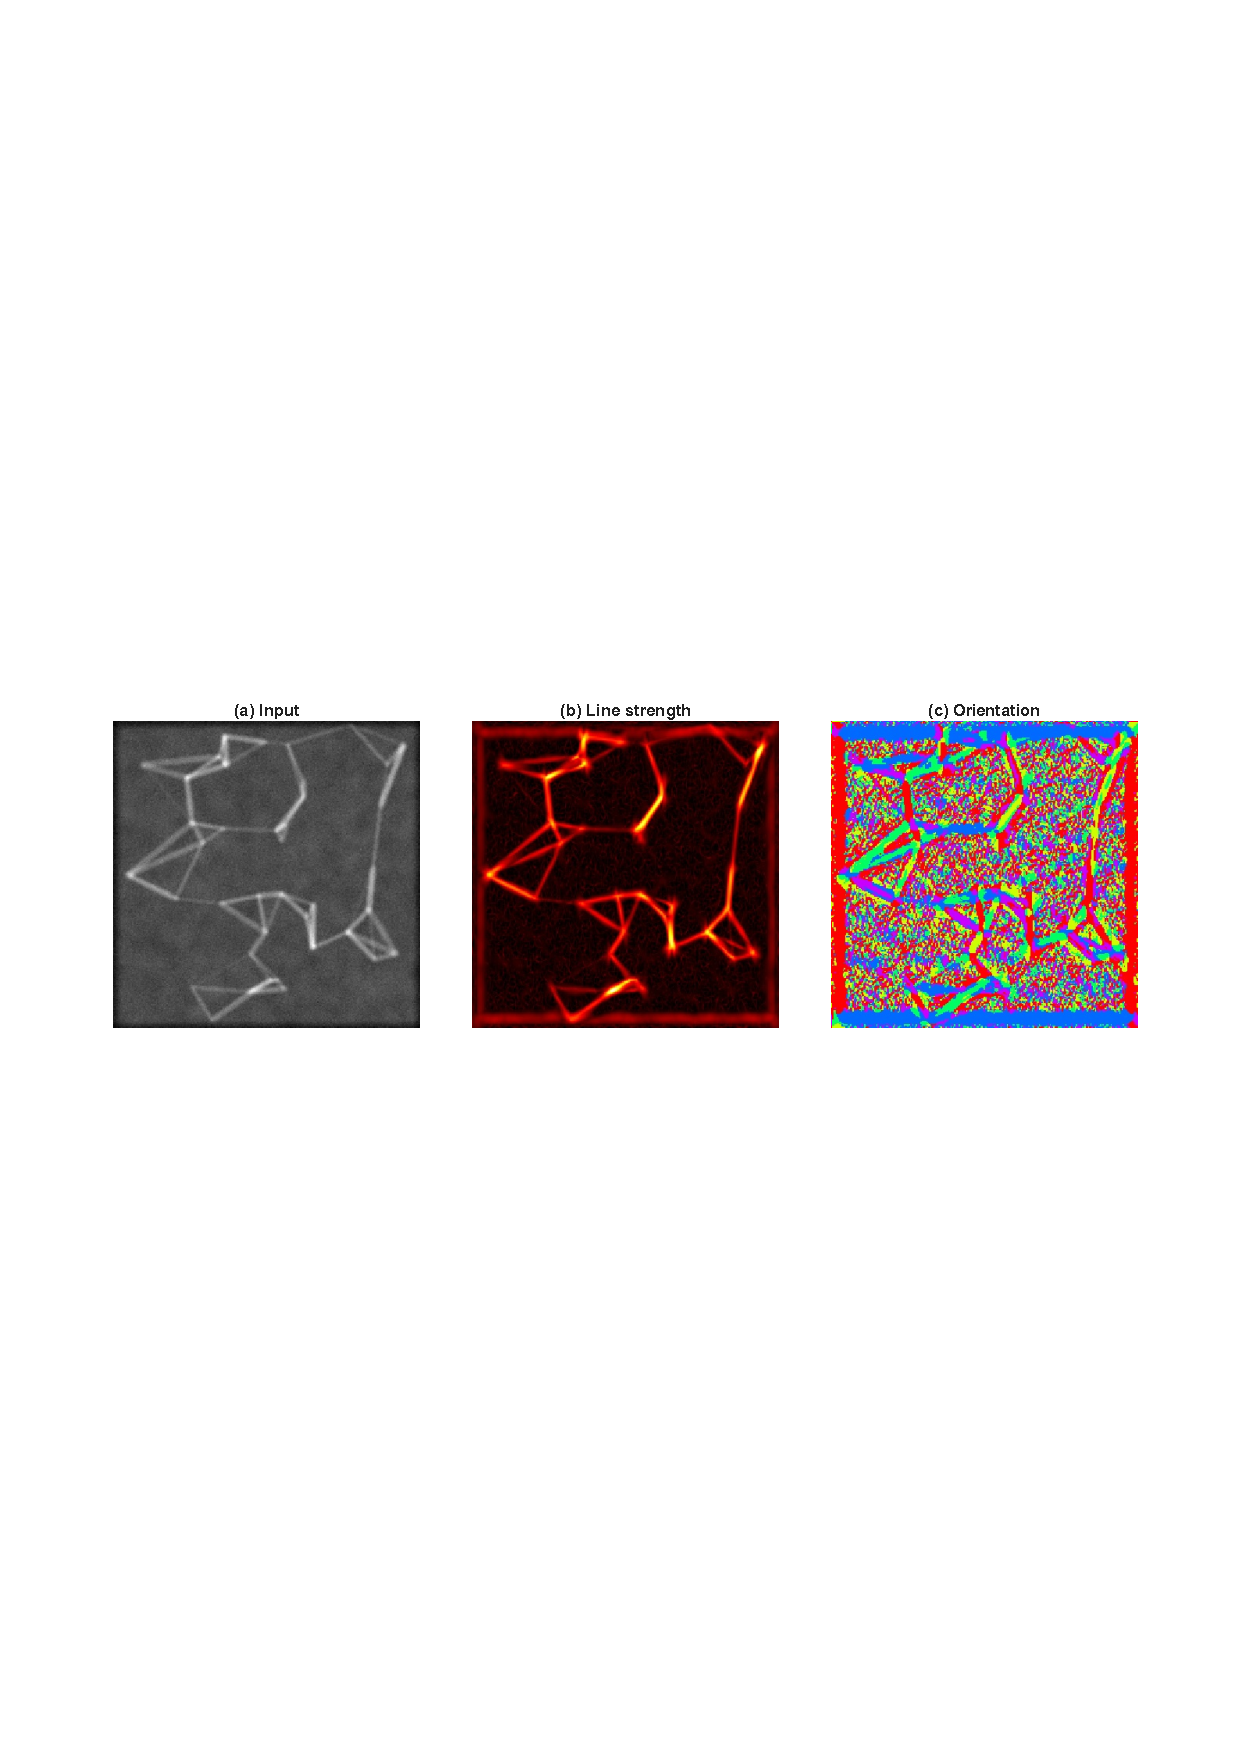
\includegraphics[width=0.9\linewidth]{figures/soagk_result.pdf}
  \caption{SOAGK line detector on the reticulate benchmark image.
  (a)~Input. (b)~Line strength map. (c)~Dominant orientation (HSV colourmap).}
\end{figure*}

\newpage

% =============================================================================
\section{Vesselness (Optimised Standalone)}
% =============================================================================

\texttt{Vesselness/src/\allowbreak{}vessel\-ness\-Filter\-2D\-Optimised.m} is an
optimised standalone implementation of the original Frangi vessel filter,
retained as a legacy reference. It implements the same Frangi (1998) algorithm
as the \texttt{'vesselness'} mode of \texttt{hessian2DFilters} but with a
streaming-max architecture (no 3-D scale stacks) and explicit precision
control.

\begin{lstlisting}
[outIm, whatScale, Direction] = ...
    vesselnessFilter2DOptimised(I, options)
%  options.FrangiScaleRange  [min max]  (default: [1 10])
%  options.FrangiScaleRatio             (default: 2)
%  options.FrangiBetaOne                (default: 0.5)
%  options.FrangiBetaTwo                (default: 15)
%  options.WhiteOnDark                  (default: true)
%  options.Precision                    (default: 'single')
\end{lstlisting}

\textbf{Note:} For new work, \texttt{hessian2DFilters} with
\texttt{'FilterType','vesselness'} is the recommended entry point, as it
provides a consistent API across all filter types and integrates
auto-scale selection via \texttt{autoLearnHessianScales}.

\begin{figure}
  \centering
  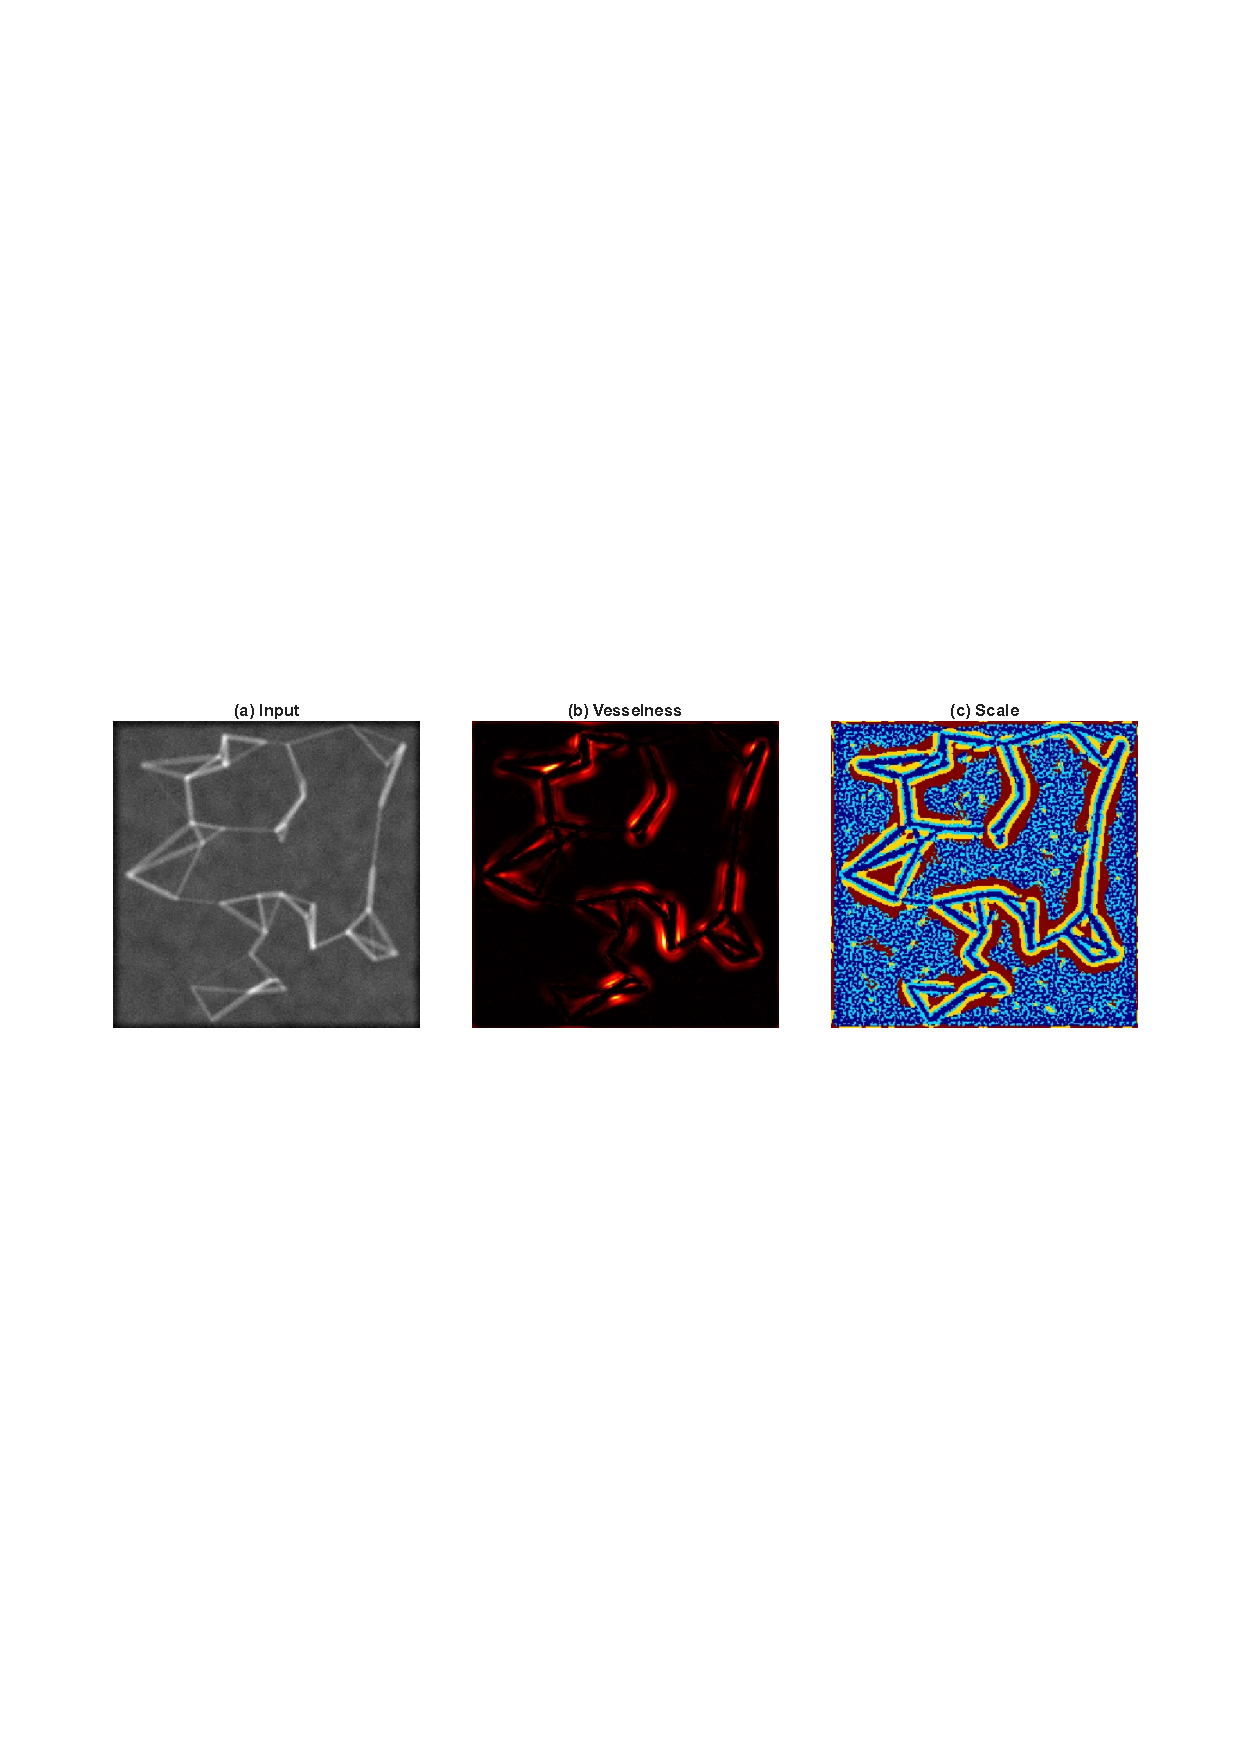
\includegraphics[width=0.9\linewidth]{figures/vesselness_optimised_result.pdf}
  \caption{Optimised standalone vesselness on the reticulate benchmark image.
  (a)~Input. (b)~Vesselness response. (c)~Scale index at maximum response.}
\end{figure}

\newpage

% =============================================================================
\section{Synthetic Benchmark Phantom}
% =============================================================================

All demos share a common synthetic image generated by
\texttt{makeReticulateTestImage(256,~256,~42)} in \texttt{Helper~functions/}.
The function produces:

\begin{itemize}
  \item a smooth background from a seeded random field,
  \item 40 random nodes connected to their 3 nearest neighbours, forming a
        reticulate (network) structure,
  \item line widths of 1--3 pixels, box-filter softened,
  \item mild Gaussian noise ($\sigma = 0.03$).
\end{itemize}

The deterministic seed (42) ensures bit-identical images across runs and
platforms. Using a shared image allows direct qualitative comparison of all
filter responses.

% =============================================================================
\section{Comparative Summary}
% =============================================================================

\begin{table}[ht]
  \centering
  \footnotesize
  \begin{tabular}{lllll}
    \toprule
    Module & Primary target & Response & Scale & Key parameters \\
    \midrule
    Hessian/vesselness  & Tubular structures   & Soft [0,1]  & Multi & $\beta$, $c$ \\
    Hessian/ridge       & Ridge lines          & Soft [0,1]  & Multi & $\alpha$ \\
    Hessian/blobness    & Isotropic blobs      & Soft [0,1]  & Multi & --- \\
    Hessian/neuriteness & Curvilinear shape    & Normalised  & Single & --- \\
    MFAT-$\lambda$      & Curvilinear (strict) & Near-binary & Multi & $\tau$, $D$ \\
    MFAT-Prob           & Curvilinear (soft)   & Probability & Multi & Beta prior \\
    Phase Congruency    & Edges \& corners     & Invariant   & Multi & $k$, $g$ \\
    Phase Symmetry      & Symmetric features   & Invariant   & Multi & polarity \\
    SOAGK               & Line segments        & Normalised  & Multi & $\rho$ \\
    Vesselness (opt.)   & Tubular (legacy)     & Soft [0,1]  & Multi & $\beta$, $c$ \\
    \bottomrule
  \end{tabular}
  \caption{Summary of filter families, their primary targets, response type,
  scale handling, and key tuning parameters.}
\end{table}

% =============================================================================
\section{Test Suite}
% =============================================================================

Each module ships with a unit test suite exercising documented mathematical
guarantees. Tests are run with \texttt{runtests('test\_<module>')} in MATLAB.

\begin{table}[ht]
  \centering
  \footnotesize
  \begin{tabular}{lll}
    \toprule
    Module & Test file & Key invariants \\
    \midrule
    Hessian & \texttt{test\_vesselness\_basic.m} & Line detection, polarity \\
            & \texttt{test\_eig2image.m} & Eigenvalue ordering \\
            & \texttt{test\_hessianEigen2D\_scale.m} & Scale normalisation \\
            & \texttt{test\_hessian\_direction.m} & Orientation accuracy \\
            & \texttt{test\_neuriteness\_*.m} (3 files) & Blob suppression, continuity \\[2pt]
    MFAT    & \texttt{TestMfat.m} & Lambda/Prob output ranges \\[2pt]
    PhaseCongruency & \texttt{test\_phasecong3Optimised.m}
            & Output ranges, determinism, precision, cache \\[2pt]
    SOAGK   & \texttt{test\_AGlineDetector.m}
            & Size, [0,1] range, line response, orientation,
              conv2/imfilter equivalence \\[2pt]
    Vesselness & \texttt{test\_vesselnessFilter2DOptimised.m}
            & Numerical agreement with reference \\
    \bottomrule
  \end{tabular}
  \caption{Unit test coverage per module. No test asserts behaviour not
  guaranteed by the underlying theory.}
\end{table}

% =============================================================================
\section{Repository Layout and Build Instructions}
% =============================================================================

\subsection{Folder Structure}

\begin{verbatim}
CurvilinearFilters_sandbox/
|-- Hessian/
|   |-- src/  engine/  neuriteness/  utils/
|   |-- demos/
|   `-- tests/  utilities/
|-- MFAT/
|   |-- src/  core/  drivers/  responses/  modifiers/  utils/
|   |-- config/
|   |-- demos/
|   `-- tests/
|-- PhaseCongruency/
|   |-- src/
|   |-- utils/
|   |-- demos/
|   `-- tests/
|-- SOAGK/
|   |-- src/
|   |-- utils/
|   |-- demos/
|   `-- tests/
|-- Vesselness/
|   |-- src/
|   |-- +vesselness/
|   |-- demos/
|   `-- tests/
|-- Helper functions/
|   `-- makeReticulateTestImage.m
`-- manual/
    |-- CurvilinearFilters.tex
    |-- figures/
    `-- demos/
        `-- demo_generateManualFigures.m
\end{verbatim}

\subsection{Generating Figures}

Before compiling the manual, run the master figure-generation script from
MATLAB:

\begin{lstlisting}
cd manual/demos
run demo_generateManualFigures
\end{lstlisting}

This script adds all module paths, runs each filter on the shared test image,
and saves PDF figures to \texttt{manual/figures/}.

\subsection{Compiling the Manual}

\begin{verbatim}
cd manual
pdflatex CurvilinearFilters.tex
pdflatex CurvilinearFilters.tex   % second pass for TOC
\end{verbatim}

% =============================================================================
\begin{thebibliography}{9}

\bibitem[Frangi et~al.(1998)]{Frangi1998}
A.~F. Frangi, W.~J. Niessen, K.~L. Vincken, and M.~A. Viergever.
\newblock Multiscale vessel enhancement filtering.
\newblock \emph{Medical Image Computing and Computer-Assisted Intervention},
1998.

\bibitem[Sato et~al.(1998)]{Sato1998}
Y.~Sato, S.~Nakajima, N.~Shiraga, H.~Atsumi, S.~Yoshida, T.~Koller,
G.~Gerig, and R.~Kikinis.
\newblock Three-dimensional multi-scale line filter for segmentation and
visualization of curvilinear structures in medical images.
\newblock \emph{Medical Image Analysis}, 2(2):143--168, 1998.

\bibitem[Lindeberg(1998)]{Lindeberg1998}
T.~Lindeberg.
\newblock Feature detection with automatic scale selection.
\newblock \emph{International Journal of Computer Vision}, 30(2):79--116, 1998.

\bibitem[Meijering et~al.(2004)]{Meijering2004}
E.~Meijering, M.~Jacob, J.-C. Sarria, P.~Steiner, H.~Hirling, and M.~Unser.
\newblock Design and validation of a tool for neurite tracing and analysis in
fluorescence microscopy images.
\newblock \emph{Cytometry Part A}, 58A:167--176, 2004.

\bibitem[Alhasson et~al.(2018)]{Alhasson2018}
H.~F. Alhasson, S.~S. Alharbi, and B.~Bhattacharyya.
\newblock 2D and 3D vascular structures enhancement via multiscale fractional
anisotropy tensor.
\newblock In \emph{ECCV Workshops (BioImage Computing)}, 2018.

\bibitem[Kovesi(1999)]{Kovesi1999}
P.~Kovesi.
\newblock Image features from phase congruency.
\newblock \emph{Videre: Journal of Computer Vision Research}, 1(3), 1999.

\bibitem[Basser et~al.(1994)]{Basser1994}
P.~J. Basser, J.~Mattiello, and D.~LeBihan.
\newblock MR diffusion tensor spectroscopy and imaging.
\newblock \emph{Biophysical Journal}, 66(1):259--267, 1994.

\end{thebibliography}

\end{document}
